\section{}

%Part A
\subsection{}
The plot for importance resampling for $n=100$ can be found in Figure \ref{fig:resample_m100}.
The plot for $n=10000$ can be found in Figure \ref{fig:resample_m10000}.

\begin{figure}
     \centering
     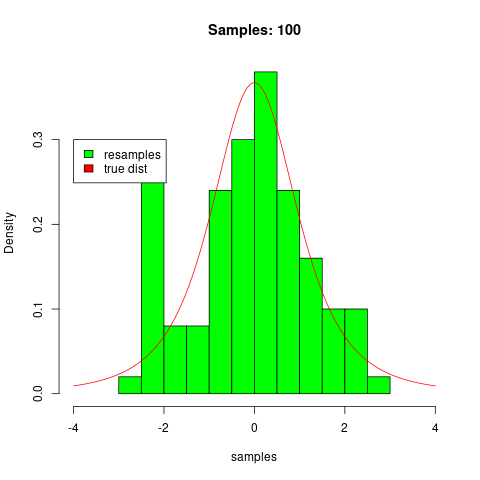
\includegraphics[width=.50\textwidth]{../code/q1/plots/resample_m100.png}
     \caption{Importance sampling. n=100}
     \label{fig:resample_m100}
\end{figure}
\begin{figure}
     \centering
     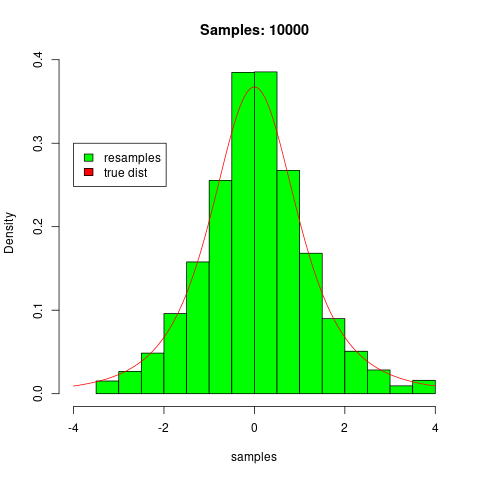
\includegraphics[width=.50\textwidth]{../code/q1/plots/resample_m10000.png}
     \caption{Importance sampling. n=100}
     \label{fig:resample_m10000}
\end{figure}


%Part B
\subsection{}
\subsubsection*{n=100}
\noindent For $n=100$, my estimate $\hat{\mu} = -0.119$.\\
For the t distribution with 3 degrees of freedom, $t_3$, the mean should be 0.\\
My $s^2$ estimate for the variance was $1.25915827778705$\\
For the $t_3$ distribution this variance is 3.

These do not seem like very good estimate so I would like to explain my calculation. 
I calculated the mean by using the dot product of my proposal samples and the normalized `weights', 
where each weight is the proposal density divided by the $t_3$ (true) density of a each sample.

For the sample variance I element-wise multiplied the samples by each corresponding weight,
then subtracted my mean estimate, square, summed, and divided by $n-1$.

These calculations seemed correct to me and my resampling looked good

\subsubsection*{n=10000}
The same caluculations as above produces $\hat{\mu} = -0.0499$ and $s^2 = 13.7920400662904$.
There was clearly something wrong with my calculation, but I could not figure out what.
My resampling plots looked good so I couldn't figure out the issue.


